\section{The Web as a platform} \label{chapter2:web-as-a-platform}

\subsection{From Operating Systems to the World Wide Web}


% With the invention of electronic computing machine, appeared the market for software applications.
% This market is not limited by marginal production cost ; software being a virtual product, the production and distribution cost for another unit is virtually null.
% The market is limited by the platform a software can be deployed on.
% The bigger the platform, the wider the market.
% There is an economically incentive to standardize and widen the platform, both for the provider, and for the consumer.
% The first platforms started as products, in competition with other products.
% Their manufacturers had economical incentive to increase their market share.
% Microsoft successfully took over the market of operating system in the 90s, and was on the edge of monopoly more than once.
% But eventually, the product is standardized, and becomes the platform.

% Before the internet, this market was limited for distribution by the physical medium.
% It takes time to burn a CD, or a floppy, and to bring it to the consummer's home.
% Sir Tim Berners Lee invented the world wide web in 1989.
% It was initially intended to share scientific documents and results.
% And it eventually became the distribution medium of choice for every virtual products, software included.
% It pushed the scalability of software distribution.

% Similarly to operating systems, Web browsers started as software products.
% They exposed innovative features to try to increase their market share.
% Among others is the ability to run scripts.
% It allows to deploy and run software at unprecedented scales.
% The web became the platform.
% Now, with web services, or Software as a Service (SaaS), the distribution medium of software is so transparent that owning a software product to have an easier access is no longer relevant.
% We explore now the different languages to write and deploy applications on the web.


\begin{wrapfigure}{r}{0.2\textwidth}
  \vspace{-27pt}
  \begin{center}
    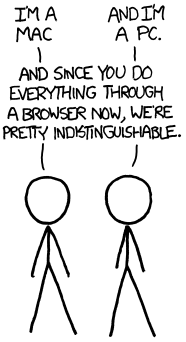
\includegraphics[width=0.18\textwidth]{../ressources/Mac-PC.png}
  \end{center}
  \vspace{-20pt}
\end{wrapfigure}

The production and distribution cost for another unit of a software application is virtually null.
The market is only limited by the platform a software can be deployed on.
The bigger the platform, the wider the market.
% There is an economical incentive to standardize and widen the platform, both for the provider, and for the consumer.
% The first platforms started as products, in competition with other products.
% Their manufacturers had economical incentive to increase their market share.
% Microsoft successfully took over the market of operating system in the 90s, and was on the edge of monopoly more than once.
% But eventually, the product is standardized, and becomes the platform.
% The market of operating system was limited for distribution by the physical medium.
% It takes time to burn a CD, or a floppy, and to bring it to the consummer's home.
Sir Tim Berners Lee invented the world wide web.
It spreads the scalability of software distribution world wide with a near zero latency.
It eventually became the main distribution medium for software, and the wider market there can possibly be.

Similarly to operating systems, Web browsers started as software products with the ability to run scripts to extend their possibilities.
% They exposed innovative features to try to increase their market share.
It led the web to become the platform, replacing operating systems.
Now, with web services, or Software as a Service (SaaS), the distribution medium of software is so transparent that owning a software product to have an easier access is no longer relevant.
It stimulates a competly new business model based on a free access for the user, while claiming value for their data.
We explore in the next paragraphs the different languages that allowed this new business model to emerge.

\subsection{The Languages of the Web}

In the 80's and early 90's, with Moore's law predicting exponential increase in hardware performance, development time became more expensive than hardware.
Higher-level languages replaced lower-level languages. %, trading perfomance for accessibility.
The economical gain in development time compensated the worsen performances.
During the web early development, most of the now popular programming languages were released, Python(1991), Ruby(1993), Java(1994), PHP(1995) and Javascript(1995).

Java, developed by Sun Microsystems, imposes itself early as a language of choice and never really decreased.
The language is executed on a virtual machine, allowing to write an application once, and to deploy it on heterogeneous machines.
The software industry quickly adopted it as its main development language.
% It is currently the second most cited language on StackOverflow, and used on Github.
% And is in the first place of many language popularity indexes.
However, because of the heavy adoption by the software industry, Java lose the hype that drove the community innovation and creativy.
It struggles to keep up with the latest trends in software development.

\textit{Python is the second best language for everything.}
It is a general purpose language, currently popular for data science.
In 2003, the release of the Django web framworks brought the language to the web development scene.

Ruby was almost unknown until the release of Rails in 2005.
With the release of this web framework, Ruby took-off and is still in active use.
% It meets the latest trends in software development.
% And it might had replaced Java if the latter had not been so well adopted in the software industry.

PHP %stands for Personal Home Page Tools.
was initially designed to build personal web pages.
It might be one of the easiest language to start web development, but even though there is some success story, it is generally unfit to grow projects to industrial size.
It is on a slow decline since a few years according to several language popularity indexes.

Since a few years, Javascript is slowly becoming the main language for web development.
It is the only choice in the browser.
Because of this unavoidable position, it became fast (V8, ASM.js) and convenient (ES6, ES7).
% It is a target for LLVM, allowing many languages to compile to Javascript, strengthening again its omnipresent position.
And since 2009, it is present on the server as well with Node.js
This omnipresence became an advantage.
It allows to develop and maintain the whole application with the same language.
% I argue that Javascript is the language of choice to prototype and maintain an application.

\subsection{Explosion of Javascript popularity}

\subsubsection{In the beginning}

Javascript was created by Brendan Eich at Netscape around May 1995, and released to the public in September.
At the time, Java was quickly adopted as the default language for web servers development, and everybody was betting on pushing Java to the client as well.
The history proved them wrong.

% When Javascript was released in 1995, the world wide web was on the rise.\ftnt{http://www.internetlivestats.com/internet-users/}
% Browsers were emerging, and started a battle to show off the best features and user experience to attract the wider public.\footnote{to get an idea of the web in 1997 : \url{http://1x-upon.com/}}
Javascript was released a scripting engine on Netscape navigator.
Microsoft released their browser Internet Explorer 3 in June 1996 with a concurrent implementation of Javascript.
At the time, because of the differences between the two implementations, web pages had to be designed for a specific browser.
This competition was fragmenting the web.
Netscape submitted Javascript to Ecma International for standardization in November 1996 to stop this fragmentation.
In June 1997, ECMA International released ECMA-262, the first specification of ECMAScript, the standard for Javascript.
A standard to which all browser should refer for their implementations.
% TODO more on the Ecma specification ?

The initial release of Javascript was designed in a rush. The version released in 1995 was finished within 10 days.
And, it was intended to be simple enough to attract unexperienced developers.
For these reasons, the language was considered poorly designed and unattractive by the developer community.

\illustration{the ugly duckling}

{\fontfamily{phv}\fontseries{l}
\fontsize{10pt}{10pt}\selectfont
Why does Javascript suck?\ftnt{http://whydoesitsuck.com/why-does-javascript-suck/}

Is Javascript here to stay?\ftnt{http://www.javaworld.com/article/2077224/learn-java/is-javascript-here-to-stay-.html}

Why Javascript Is Doomed.\ftnt{http://simpleprogrammer.com/2013/05/06/why-javascript-is-doomed/}

Why JavaScript Makes Bad Developers.\ftnt{https://thorprojects.com/blog/Lists/Posts/Post.aspx?ID=1646}

JavaScript: The World's Most Misunderstood Programming Language\ftnt{http://www.crockford.com/javascript/javascript.html}

Why Javascript Still Sucks\ftnt{http://www.boronine.com/2012/12/14/Why-JavaScript-Still-Sucks/}

10 things we hate about JavaScript\ftnt{http://www.infoworld.com/article/2606605/javascript/146732-10-things-we-hate-about-JavaScript.html}

Why do so many people seem to hate Javascript?\ftnt{https://www.quora.com/Why-do-so-many-people-seem-to-hate-JavaScript}
}

But things evolved drastically since.
One of the reason for the success of Javascript is the \textit{View Source} menu that reveals the complete source code of any web site.
% The success of Javascript is due to many factors ; maybe the most important of all is the \textit{View Source} menu that reveals the complete source code of any web application.
% \textit{The view source menu is the ultimate form of open source}\ftnt{http://blog.codinghorror.com/the-power-of-view-source/}.
It allows the community to pick, improve and reproduce the best techniques \ftnt{http://blog.codinghorror.com/the-power-of-view-source/}.
% It brought open source and collaborative development to the web.
Another reason is that all web browsers include a Javascript interpreter, making Javascript the most ubiquitous runtime in history \cite{Flanagan2006}.
% Every browser include development tools for Javascript, making it the most ubiquitous development environment, as well.
Javascript is distributed freely, with all the tools needed to reproduce and experiment on the largest communication network in history.
Anybody can seize this opportunity to incrementally build and share the best tools they can.
This open collaboration is the reason for the popularity of Javascript on the Web.

% When such a language is distributed freely with the tools to reproduce and experiment on every piece of code.
% And its distribution is carried during the expansion of the largest communication network in history.
% Then an entire generation seizes this opportunity to incrementally build and share the best tools they can.
% This collaboration is the reason for the popularity of Javascript on the Web.
% When a language is released, available freely at a world wide scale, and simple enough to be handled by a generation of teenager inspired by the technology hype, it produce an effervescent community around what is now one of the most popular and widely used programming language.

\subsubsection{Rising of the unpopular language}

Javascript started as a programming language to implement short interactions on web pages.
The best usage example was to validate some forms on the client before sending the request to the server.
This situation hugely improved since the beginning of the language.
Nowadays, there is a lot of web-based application replacing desktop applications, like mail client, word processor, music player, graphics editor…

% There is now proportionally more software services released to the public as web-based application than desktop clients. \nt{TODO need source}

ECMA International released several version in the few years following the creation of Javascript.
% The first and second version, released in 1997 and 1998, brought minor revisions to the initial draft.
The third version %, released in the late 1999,
contributed to give Javascript a more complete and solid base as a programming language.
From this point on, the consideration for Javascript kept improving.

%An important reason for this reconsideration started in 2005.
In 2005, James Jesse Garrett released \textit{Ajax: A New Approach to Web Applications}, a white paper coining the term Ajax \cite{Garrett2005}.
This paper explains the advantage on user experience of this technique.
% Ajax stands for Asynchronous Javascript And XML.
It uses Javascript to reload the content inside a web page without requesting a full page from the server, but only the new content.
Javascript rose outside of superficial user interactions.
Indeed, it allows to develop richer applications inside the browser, from user interactions to network communications.
%, while keeping all the advantages of web-based applications.
The first web applications to use Ajax were Gmail, and Google maps\footnote{A more in-depth analysis of the history of Ajax, given by late Aaron Swartz \url{http://www.aaronsw.com/weblog/ajaxhistory}}.

% The third version of ECMAScript had been released, and it was homogeneously supported in the browsers.
% , the DOM, and the \texttt{XMLHttpRequest} method, two components on which ... relies, 
Because of the difference of implementations, AJAX still present heterogeneous interfaces among browsers.
% Around this time, the Javascript community started to emerge.
Around this time, the community realeased Javascript framework with the goal to straighten this differences.
Prototype\ftnt{http://prototypejs.org/} and DOJO\ftnt{https://dojotoolkit.org/} are early famous examples, and later jQuery\ftnt{https://jquery.com/} and underscore\ftnt{http://underscorejs.org/}.
These frameworks took some responsibilities to the large success of Javascript and of the web technologies.

In the meantime, in 2004, the Web Hypertext Application Technology Working Group\ftnt{https://whatwg.org/} was formed to work on the fifth version of the HTML standard.
The name is misleading, it is really about giving Javascript superpowers.
% This new version provide new capabilities to web browsers, and a better integration with the native environment.
It features geolocation, file API, web storage, canvas drawing element, audio and video capabilities, drag and drop, browser history manipulation, and many mores.
% It gave Javascript the missing interfaces to become the environment required to develop rich application in the browser.
% The first public draft of HTML 5 was released in 2008, and the fifth version of ECMAScript was released in 2009.
The releases of HTML5 and ECMAScript 5, in 2008 and 2009, represent a mile-stone in the development of web-based applications.
Around the same time, Google released V8 for its browser Chrome.
It is a Javascript interpreter improving drastically the execution performance. % with a just-in-time compiler.
Javascript became the programming language of this rising application platform.

Taking advantage of this increase in performance, Node.js pushed Javascript to the server as well in 2009.
% Javascript was initially proposed to develop user interfaces.
Javascript is often associated with an event-based paradigm to react to concurrent user interactions.
This event-based paradigm proved to be also very efficient to react to concurrent requests of a web server.
Javascript is now the only language to build a complete web service, from the client to the server.
% I will present this event-based paradigm in the next section.

% Javascript, and web technologies are also used outside the web.
% NW.js\ftnt{https://github.com/nwjs/nw.js} and electron\ftnt{https://github.com/atom/electron} are two solutions to deploy application built with web technologies.
% They use Node.js and Chromium.
% The Atom text editor\ftnt{https://atom.io/}, Popcorn Time\ftnt{https://popcorntime.io/} and Light Table\ftnt{http://lighttable.com/} are example of such applications.
% However, if web applications are common choice for web service client on the desktop, HTML5 is not yet widely accepted as ready to build complete application on mobile, where performance and design are crucial.
% Indeed web-technologies are often not as capable, and well integrated as native technologies.
% But even for native development, Javascript seems to be a language of choice.
% An example is the React Native Framework\ftnt{https://facebook.github.io/react-native/} from Facebook, which allow to use Javascript to develop native mobile applications.
% They prone the philosophy \textit{"learn once, write anywhere"}, in opposition to the usual slogan \textit{"write once, run everywhere"}.\footnote{Used firstly by Sun for Java, but then stolen by many others}
% Another example is Gnome-shell. It uses Javascript to build its interface, and extensions.
% PhoneGap (Cordova) is a huge effort toward bringing web technologies to the mobile.




\begin{figure}

\newcommand{\event}[3][10pt]{\chronoevent[markdepth=-#1]{#2}{#3}}
\setupchronoevent{textstyle=\scriptsize,datestyle=\tiny\bf,datesseparation=/,conversionmonth=false}
% \usr\share\texmf-dist\tex\generic\chronosys\chronosyschr.tex:533 +>
% \vspace{-6pt} % I added this line because the space between date and text is too large for scriptsize font.

\startchronology[align=left, startyear=1994,stopyear=2016, height=0pt, startdate=false, stopdate=false, arrow=false, box=true]
%
\chronograduation[event][dateselevation=10pt]{2}


\event[35pt]  {06/2015}     {ECMAScript v6.0}
\event[10pt]  {14/01/2015}  {io.js}
\event[110pt] {06/2011}     {ECMAScript V5.1}
\event[85pt]  {12/2009}     {ECMAScript v5.0}
\event[60pt]  {27/06/2009}  {Node.js}
\event[35pt]  {02/09/2008}  {V8}
\event[10pt]  {22/01/2008}  {HTML5 public draft}
\event[10pt]  {04/06/2004}  {WHATWG}
\event[110pt] {12/1999}     {ECMAScript v3.0}
\event[85pt]  {06/1998}     {ECMAScript v2.0}
\event[60pt]  {06/1997}     {ECMAScript v1.0}
\event[35pt]  {11/1996}     {ECMA Standardization}
\event        {05/1995}     {Javascript Creation}



\stopchronology
\end{figure}

\subsubsection{Current situation}

\cit{When JavaScript was first introduced, I dismissed it as being not worth my attention. Much later, I took another look at it and discovered that hidden in the browser was an excellent programming language.}{Douglas Crockford}

% \cit{JavaScript is the world's most ubiquitous computing runtime.}{John Lam}



% I want to say that Javascript took off because it was carried by the open source community.
% The goal is to introduce the following facts : JS is widely used in the open source community.
% I need to find the argument saying that open source is taking over closed sources : Javascript / open source is taking over Java / closed source.

% TO READ :
% http://www.javaworld.com/article/2077224/learn-java/is-javascript-here-to-stay-.html
% http://blog.codinghorror.com/the-power-of-view-source/
% http://blog.codinghorror.com/javascript-the-lingua-franca-of-the-web/
% http://shaver.off.net/diary/2007/05/10/the-high-cost-of-some-free-tools/


% This success is obvious on the web and in the open source communities.
The rise of Javascript is obvious on the web and the open source communities.
It also seems to be rising in the software industry.
But it is difficult to give an accurate representation of the situation because the software industry often try to keep an edge by keeping a fog of war.
In the following paragraphs, I report some indexes that represent the situation globally, both in the open source community and in the more opaque software industry.
% More detailed informations are available section \ref{appendix:langpop}.

\paragraph{Available resources}

% The TIOBE Programming Community index is a monthly indicator of the popularity of programming languages.
According to the TIOBE Programming Community index, Javascript ranks 8th on this index, as of April 2015, and it was the most rising language in 2014.
This index measure of the popularity of a programming language with the number of results on many search engines.
% The results contains the resources and traces of the activity around the language that are used as a measure of the popularity of a programming language.
However, the number of pages doesn't represent the number of readers.
This measure is controversial, and might not be representative.

Alternatively, Javascript ranks 7th on the PYPL, as of October 2015.
The PYPL index is based on Google trends to measure the number of requests on a programming language.
% This index seems to be more accurate, as it depicts the actual interest of the community for a language.
However, it is not representative as it doesn't take all the available resources into account.

From these indexes, the major programming language is Java, and then C/C++, C\# and Python.
These languages are still the most widely taught, and used to write softwares.
% But Javascript is rising to become an important language as well.

\paragraph{Developers collaboration platforms}

Online tools of collaboration gives an indicator of the number of developers and project using certain languages.
% A different indicator of the popularity of a language is the number of developers and projects using it.
Javascript is the most used language on \textit{Github}, the most important collaborative development platform, with around 9 millions users.
It represents more than 320 000 repositories, while the second language is Java with more than 220 000 repositories.

% https://github.com/blog/2047-language-trends-on-github
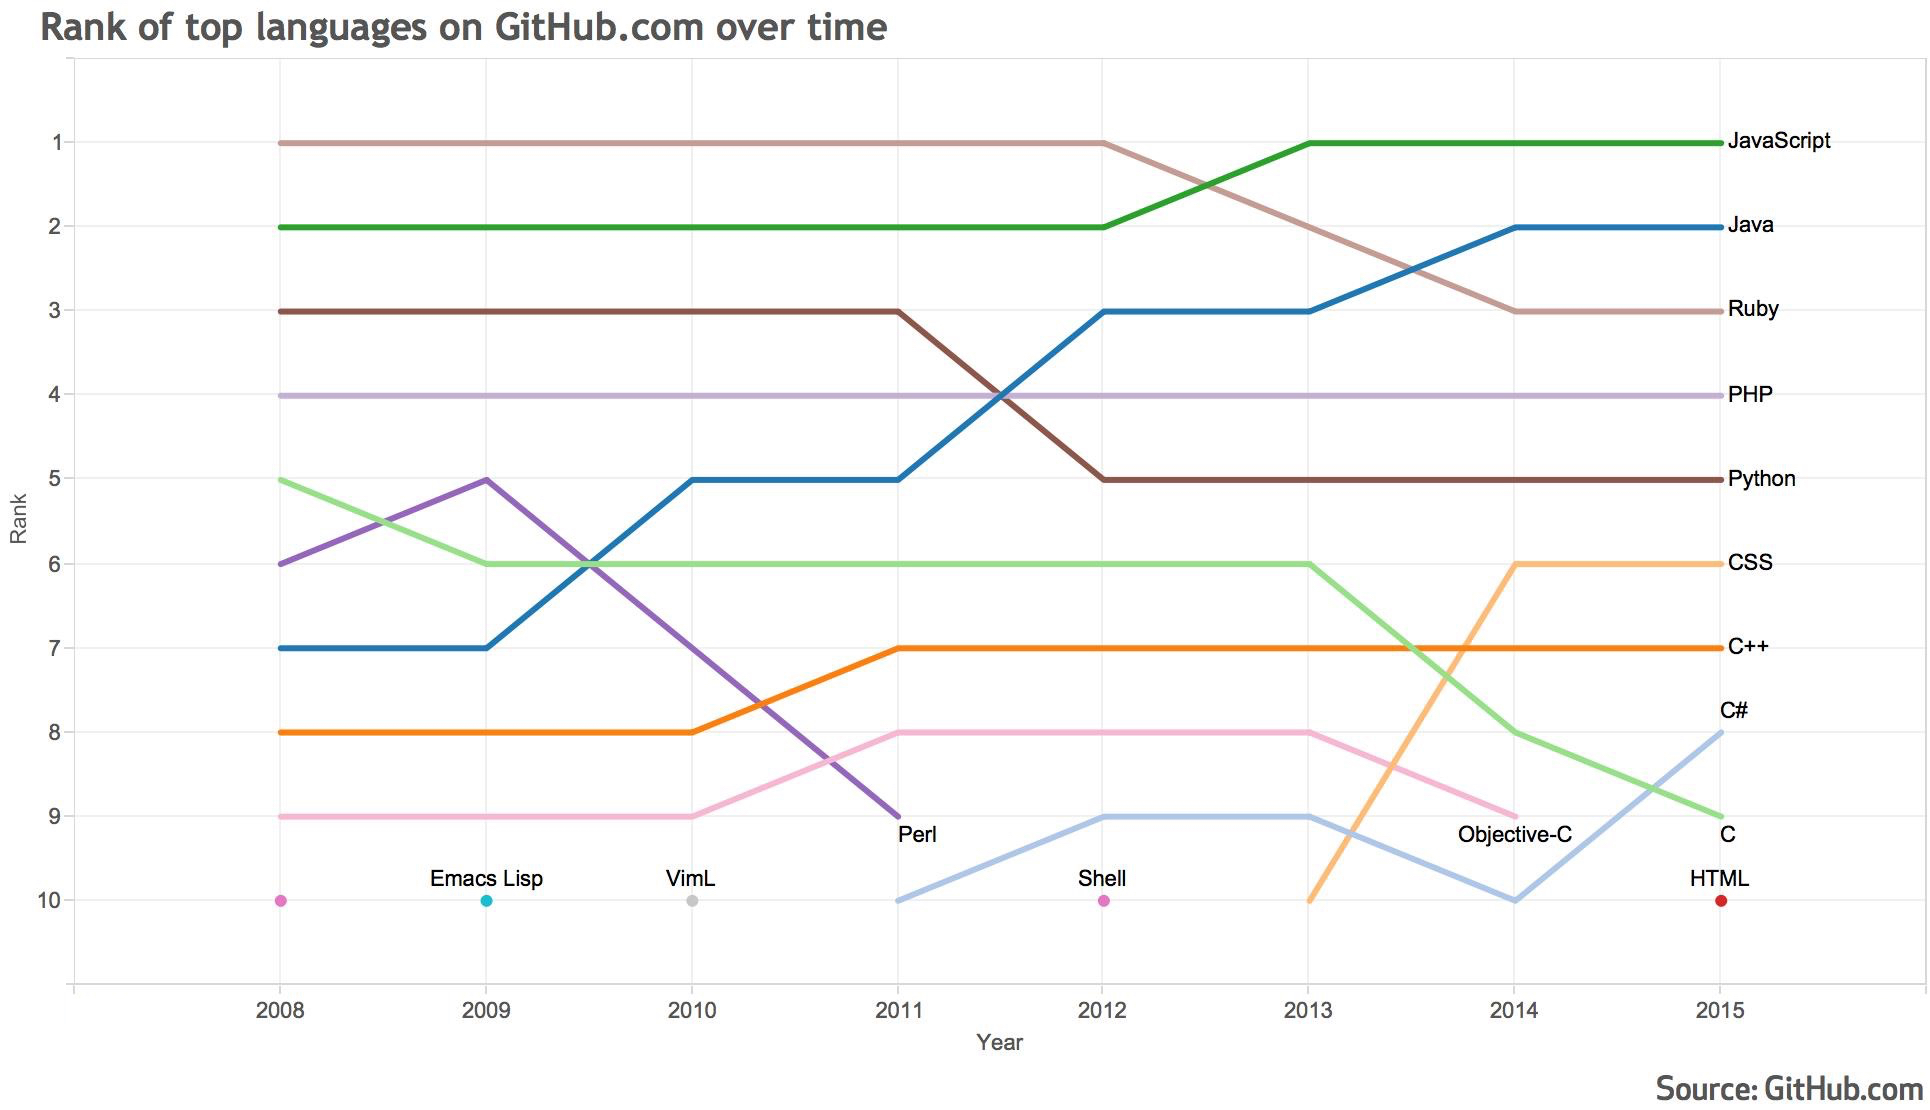
\includegraphics[width=0.9\linewidth]{../../data/js-trends/github-ranks}


Javascript is the language the most cited on \textit{StackOverflow}, the most important Q\&A platform for developers.
It is a good representation of the activity around a language.
Javascript represent more than 960 000 questions, while the second is Java with around 940 000 questions.

According to \textit{Black Duck Software}, Javascript is the second language used in open source projects.
C is first, C++ third and Java fourth.
These four languages represent about 80\% of all programming language usage in open source communities.

% Black Duck Software helps companies streamline, safeguard, and manage their use of open source.
% For its activity, it analyzes 1 million repositories over various forges, and collaborative platforms to produce an index of the usage of programming language in open source communities.
% Javascript ranks second.

\nt{TODO redo this graph, it is ugly.}
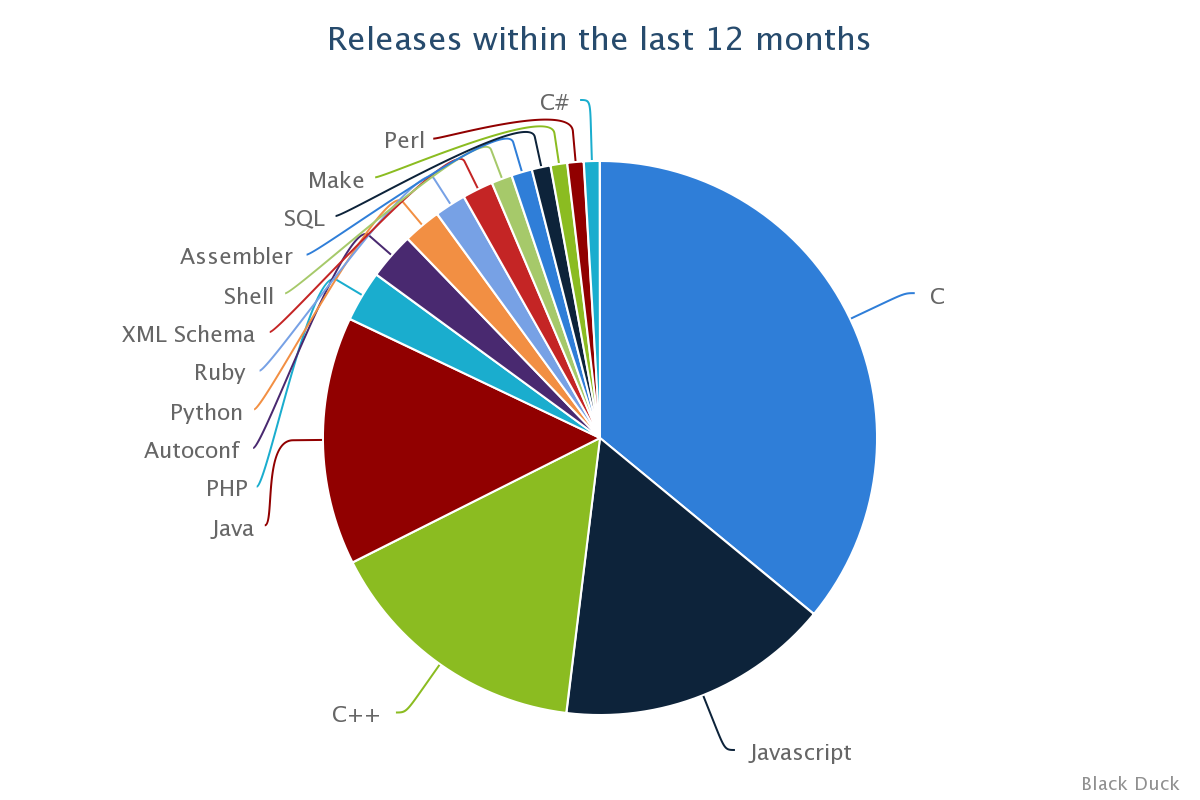
\includegraphics[width=0.9\linewidth]{../../data/js-trends/black-duck-15}

% \begin{figure}[h!]
% \begin{tikzpicture}
% [
%     pie chart,
%     slice type={c}{gray1},
%     slice type={js}{red},
%     slice type={cpp}{gray2},
%     slice type={java}{gray3},
%     slice type={php}{gray4},
%     slice type={autoconf}{gray5},
%     slice type={python}{gray6},
%     slice type={ruby}{gray1},
%     slice type={xml}{gray2},
%     slice type={sh}{gray3},
%     slice type={asm}{gray4},
%     slice type={sql}{gray5},
%     slice type={make}{gray6},
%     slice type={perl}{gray1},
%     slice type={csharp}{gray2},
%     pie values/.style={font={\small}},
%     scale=2
% ]

% \pie{}{%
%   34.80/c,%
%   15.45/js,%
%   15.13/cpp,%
%   14.02/java,%
%   2.87/php,%
%   2.65/autoconf,%
%   2.15/python,%
%   1.77/ruby,%
%   1.73/xml,%
%   1.18/sh,%
%   1.16/asm,%
%   1.07/sql,%
%   0.94/make,%
%   0.92/perl,%
%   0.90/csharp,%
% }

% \legend[shift={(1.3cm,0.9cm)}]{%
%   {C}/c,%
%   {Javascript}/js,%
%   {C++}/cpp,%
%   {Java}/java,%
%   {PHP}/php,%
%   {Autoconf}/autoconf,%
%   {Python}/python,%
%   {Ruby}/ruby,%
%   {XML Schema}/xml,%
%   {Shell}/sh,%
%   {Assembler}/asm,%
%   {SQL}/sql,%
%   {Make}/make,%
%   {Perl}/perl,%
%   {C\#}/csharp,%
% }
% \end{tikzpicture}
% \caption{Compilation results distribution}
% \end{figure}

\paragraph{Jobs}

The actors of the software industry tends to hide their activities trying to keep on edge on the competition.
All these previous metrics are representing the visible activity about programming language, but are barely representative of the software industry.
The trends on job openings give some hints on the direction the software industry is heading towards.
Javascript is the third most wanted skill, according to \textit{Indeed}, right after SQL and Java.
And over the last 5 yeats, Javascript almost closed the gap with the first and second position.
% The job searching platform \textit{Indeed} provides some trends over its database of job propositions.
% Javascript developers ranked at the third position, right after SQL and Java developers.
% Over the 5 last years, the number of job position for Javascript developers increased so as to almost close the gap with Java.
Moreover, according to \textit{breaz.io}, Javascript developers get more opportunities than any other developers.
This position indicate that Javascript is increasingly adopted in the software industry.

\nt{TODO redo this graph, it is ugly.}
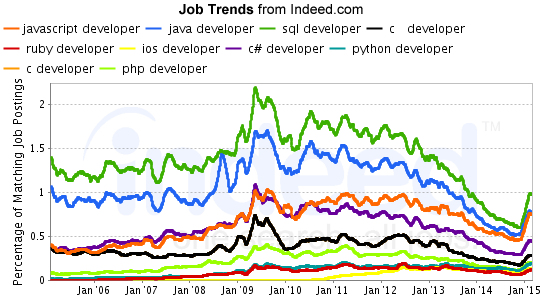
\includegraphics[width=0.9\linewidth]{../../data/js-trends/jobgraph}

\paragraph{}

All these metrics represent different faces of the current situation of the Javascript adoption in the developer community.
It is widely used in open source projects, everywhere on the web, and in the software industry.
With the evolution of web applications development and increased interest in this domain, Javascript is assuredly one of most important language in the times to come.

I just presented the languages used to build web applications.
In the next section, I present the realities and technical challenges to assure their performance against billions of users.